\documentclass[11pt]{article}
\usepackage[margin=1in]{geometry}
\usepackage{graphicx}
\usepackage{caption}
\usepackage{amsmath}
\usepackage{hyperref}

\newcommand{\figsource}[1]{\caption*{\footnotesize Source: \texttt{\detokenize{#1}}}}

\title{Eight-Code Head-Echo Matched-Filter Test}
\author{}
\date{\today}

\begin{document}
\maketitle

\section*{Purpose}

This report keeps the eight-code head-echo processing test separate from the
article figures.  The article products are not replaced by this run.  The test
uses the existing linear head-echo trajectory as the a priori range--Doppler
seed and evaluates a single Clinton head-echo patch at 0.400 s after
18:06:20 UTC.

\section*{Processing Settings}

\begin{itemize}
  \item Coherent integration length: 8 code periods.
  \item Incoherent sum: 8 spectra, stepped by 1 code period.
  \item 2-D Fourier-domain notch period: 8 Doppler bins.
  \item Gaussian smoothing: 4 pixels in range and 8 pixels in Doppler.
  \item Test station and time: Clinton, 0.400 s after 18:06:20 UTC.
\end{itemize}

\begin{figure}[htbp]
  \centering
  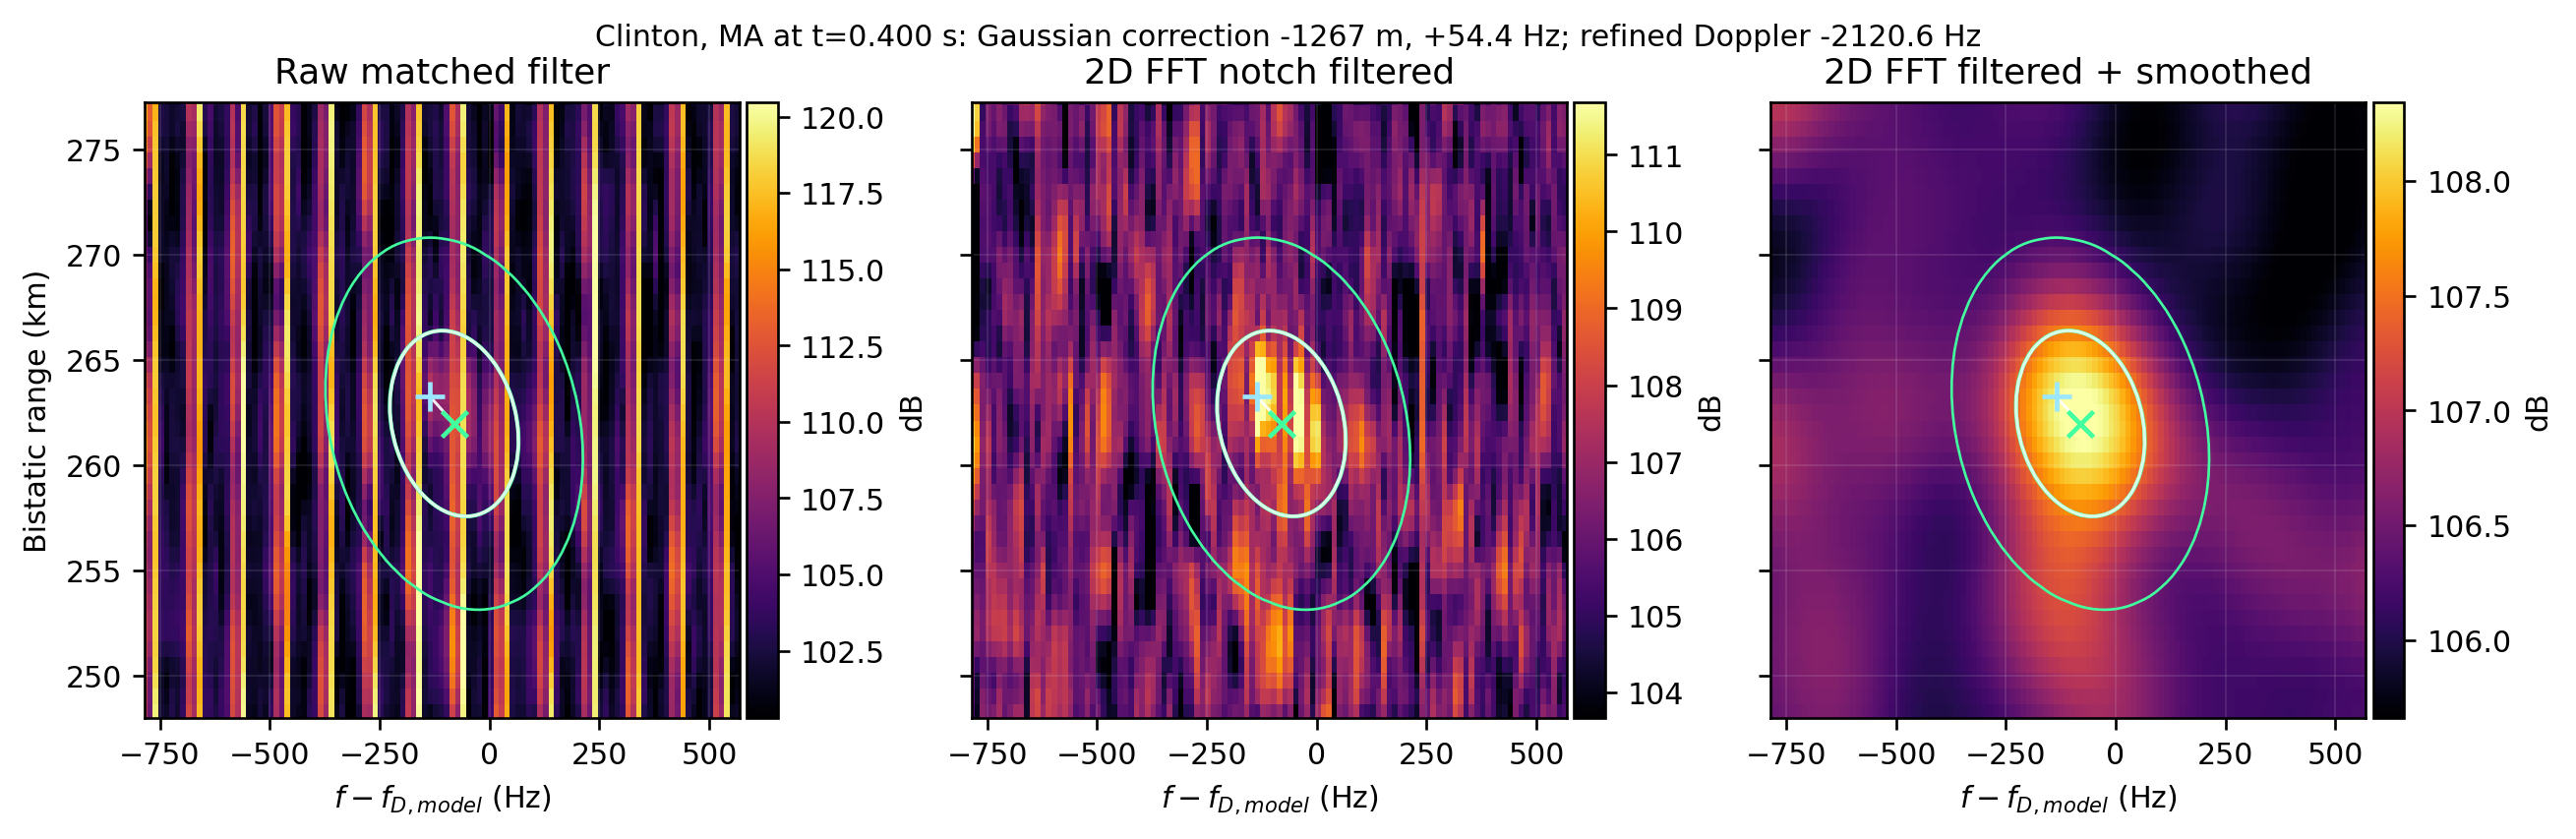
\includegraphics[width=\linewidth]{figures/head_echo_gaussian_2dfft_example_clinton_t040_ncoh8.png}
  \caption{Example Clinton range--Doppler matched-filter patch at 0.400 s after
  18:06:20 UTC using the eight-code head-echo test processing.  The panels show
  the original matched-filter image, the two-dimensional Fourier-domain
  notch-filtered image at the original resolution, and the notch-filtered image
  after zero-shift Gaussian smoothing with four-pixel range and eight-pixel
  Doppler standard deviations.  The blue plus marks the range--Doppler seed
  from the existing linear head-echo trajectory selection; the green cross and
  contours show the correlated two-dimensional Gaussian fit to the smoothed
  patch.  The white segment shows the correction from the seed to the fitted
  head-echo center.}
  \figsource{reports/generate_head_echo_gaussian_example.py}
  \label{fig:coh8-head-gaussian-example}
\end{figure}

\begin{figure}[htbp]
  \centering
  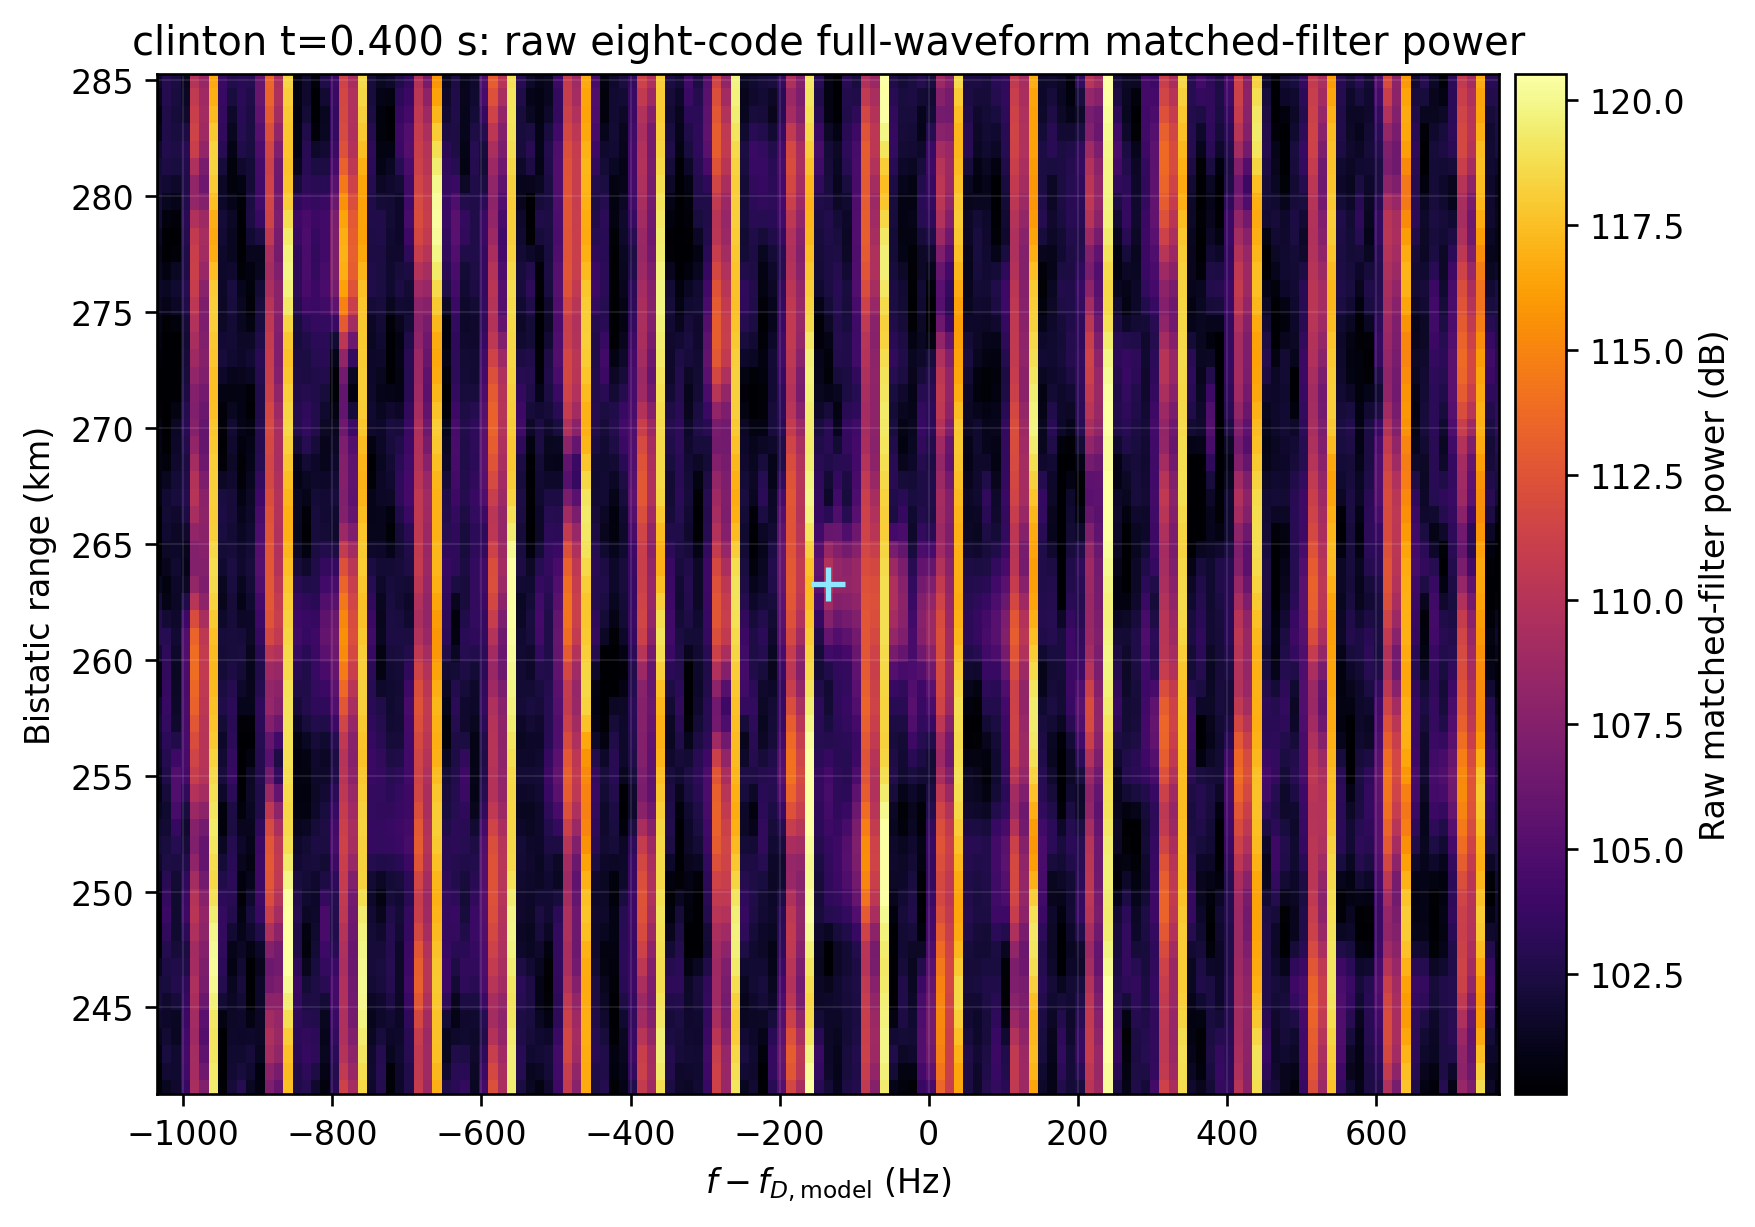
\includegraphics[width=0.92\linewidth]{figures/coh8_full_waveform_raw_match_clinton_t040.png}
  \caption{Raw Clinton range--Doppler matched-filter power at 0.400 s after
  18:06:20 UTC using the eight-code full-waveform matched-filter calculation.
  No two-dimensional Fourier-domain notch, Gaussian smoothing, median division,
  or background subtraction has been applied.  The blue plus marks the
  range--Doppler seed from the existing linear head-echo trajectory selection.
  The Doppler bin spacing is 12.5 Hz, so the repeated-code ambiguity period of
  100 Hz corresponds to eight Doppler bins.}
  \figsource{reports/plot_coh8_full_waveform_match_function.py}
  \label{fig:coh8-raw-full-waveform-match}
\end{figure}

\begin{figure}[htbp]
  \centering
  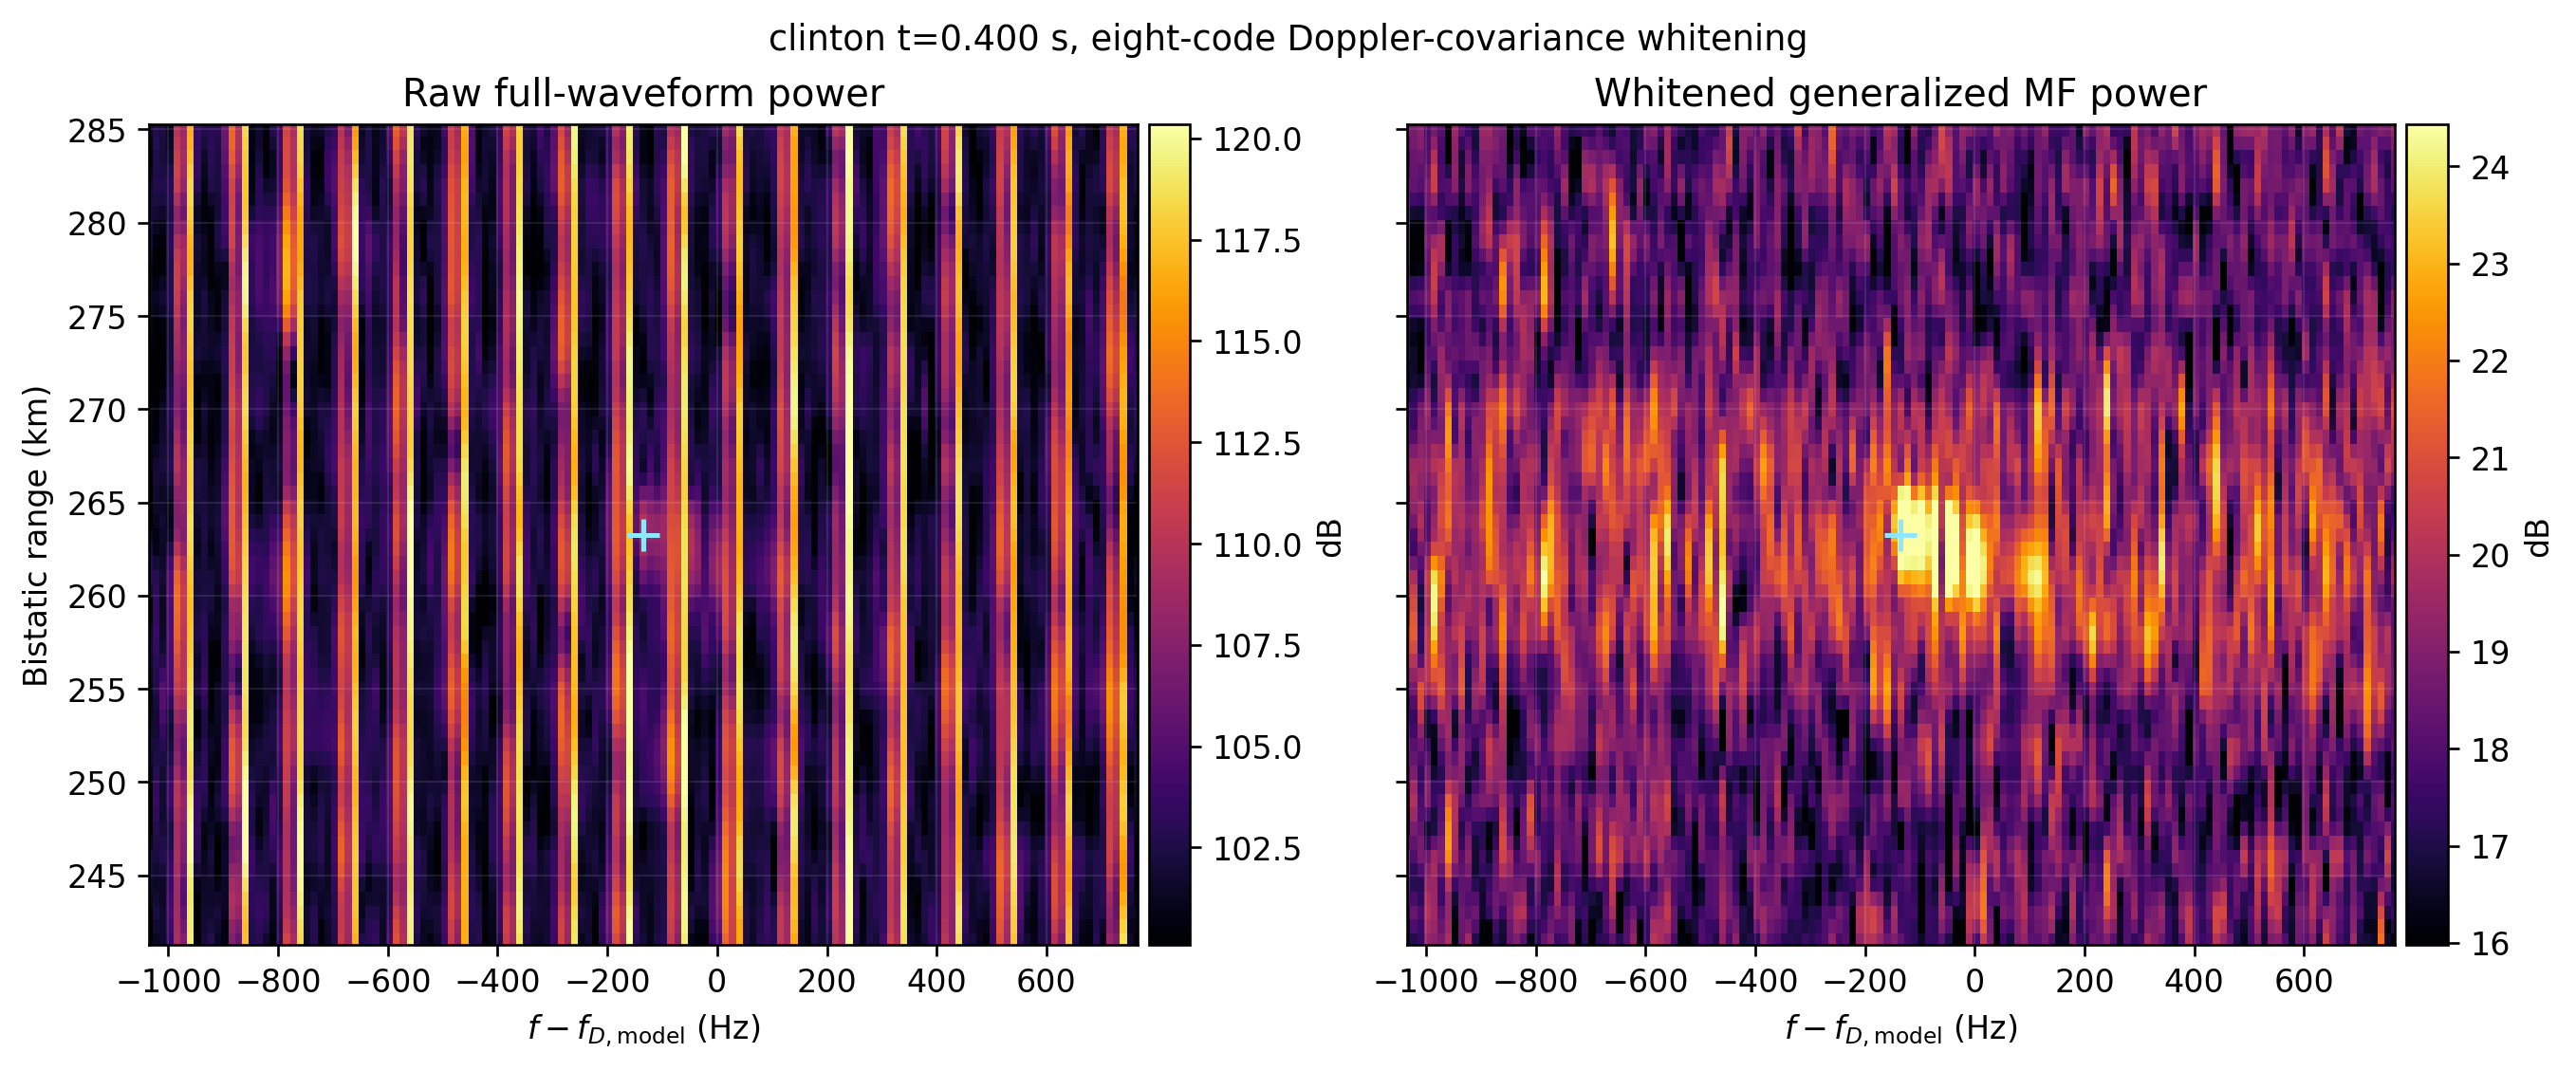
\includegraphics[width=\linewidth]{figures/coh8_whitened_match_clinton_t040_shrink002.png}
  \caption{Eight-code generalized matched-filter whitening test for the same
  Clinton head-echo patch.  The left panel repeats the raw full-waveform
  matched-filter power.  The right panel estimates the complex Doppler-bin
  covariance from off-head ranges at least 8 km away from the seed range and
  applies the inverse square-root covariance before power formation.  The
  covariance estimate uses 0.02 diagonal shrinkage.  This suppresses the
  repeated-code vertical stripe mode while retaining the localized head-echo
  blob near the trajectory seed.}
  \figsource{reports/generate_coh8_whitened_match_diagnostic.py}
  \label{fig:coh8-whitened-match}
\end{figure}

\section*{Single-Patch Result}

For this Clinton test patch, the seed range is 263.250 km and the seed Doppler
residual is \(-134.6\) Hz relative to the model.  The fitted center is
261.983 km with residual Doppler \(-80.2\) Hz, corresponding to a correction of
\(-1267\) m and \(+54.4\) Hz.

For the off-head background ranges in the raw match function, the standard
deviation of the column-median Doppler structure is 5.51 dB.  After covariance
whitening with 0.02 diagonal shrinkage, the same column-median standard
deviation is 0.33 dB.  Relative to the off-head residual image variation, the
stripe ratio drops from 0.97 to 0.28.

\end{document}
